\section{Introduction}
\label{sec:intro}

On 16 October 2026, Sreeram Kannan compared two circuit searches for elliptic-curve point addition in a public post \citep{kannan2026post}:
``anons beat anthropic by 2x / anthropic gets 21M gates at 843 qubits / ecdsa.fail gets 11.9M gates at 843 qubits.''
The next day Kydo replied that this was ``also a good case study of how cross modal pollination might produce better results'' \citep{kydo2026reply}.
Figure~\ref{fig:posts} shows both posts.

\begin{figure}[t]
\centering
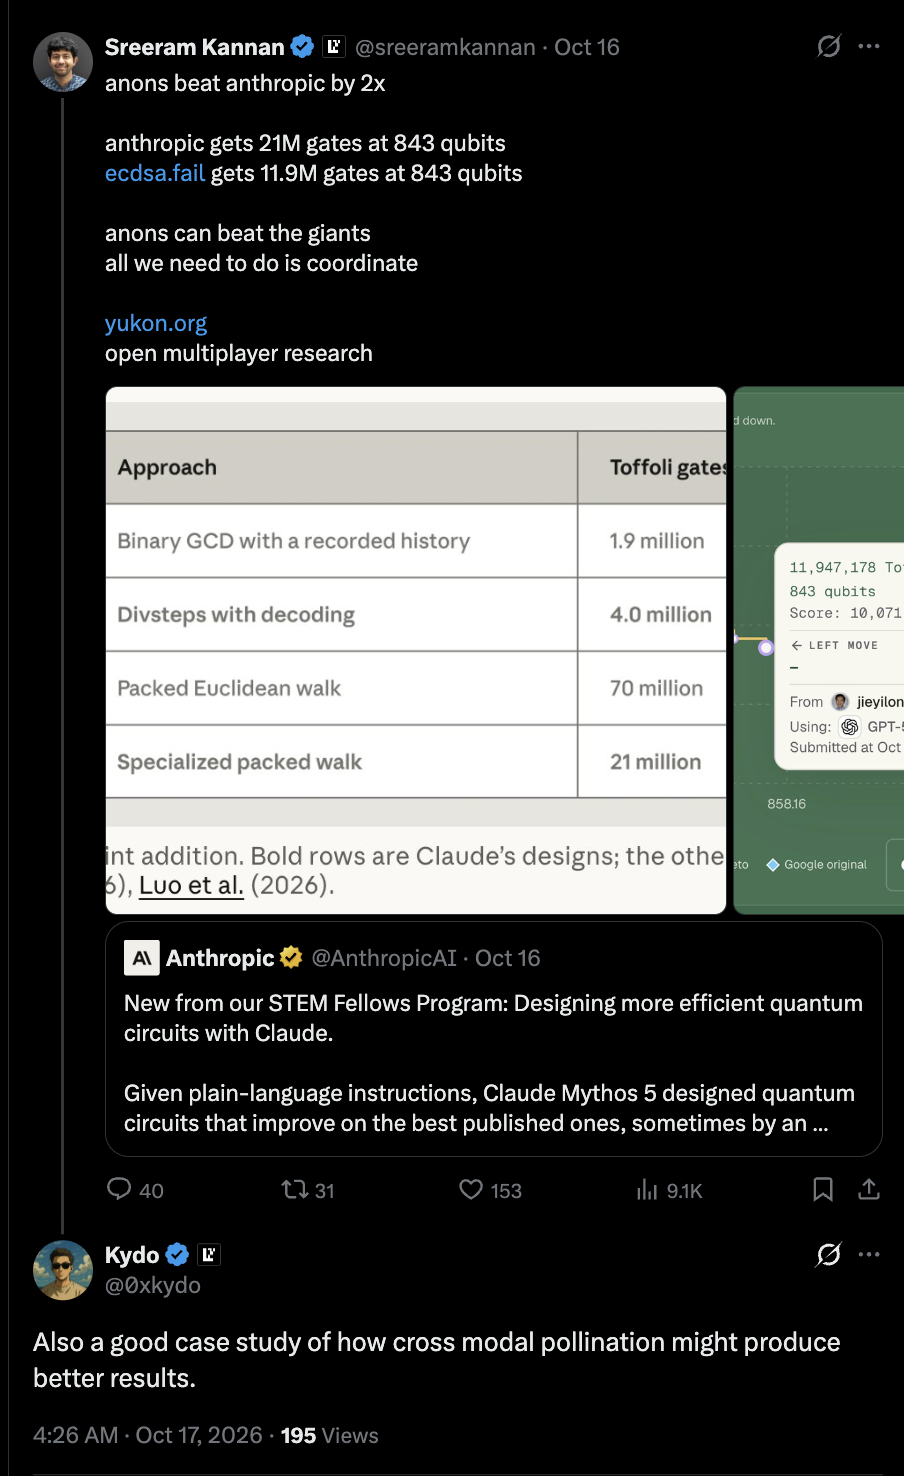
\includegraphics[width=0.46\linewidth]{figures/motivating_posts.png}
\caption{The post and reply that motivated this study, as displayed on X: the post by Sreeram Kannan on 16 October 2026, quoting Anthropic's announcement, and the reply by Kydo on 17 October 2026 \citep{kannan2026post,kydo2026reply}. The 843-qubit, 11.9M-gate point it quotes is traced in Section~\ref{sec:case843}.}
\label{fig:posts}
\end{figure}

The two searches differ in how they were organised.
The first is the evolutionary framework of \citet{gu2026discovering}, in which a single model, Claude Mythos~5, proposes circuit-generating programs inside OpenEvolve and an independent evaluator scores them.
One of its authors lists an Anthropic affiliation and another the Anthropic STEM Fellows Program.
Its Table~S3 reports a specialised Euclidean point adder at 843 qubits and, in Supplementary Section~II.2, 20.5 million Toffoli gates.
The second is ECDSA.Fail, an open leaderboard on which more than one hundred participants, each choosing their own models and tools, submitted improvements to a shared reversible circuit \citep{long2026ecdsafail}.
The two gate counts are not measured the same way.
Table~S3 of \citet{gu2026discovering} counts reversible cleanup and excludes storage or lookup used to supply the classical addend.
ECDSA.Fail scores the average executed Toffoli count over a submission-dependent set of Fiat--Shamir inputs \citep[\S6]{long2026ecdsafail}.
I use the comparison only as motivation, and nothing in this paper depends on it.

Kydo's reply names a mechanism that the ECDSA.Fail paper also describes, in prose, at four places.
Its \S4.1 says that ``independent branches using different models, tools, backgrounds, and objectives also make the search resilient to plateaus.''
Its \S4.3.2 reports that agents ``from different model families (e.g.\ GPT, Claude, Grok, GLM, and Kimi) sometimes reviewed one another's conclusions,'' and that watcher agents, which compared adjacent public submissions and summarised the transferable techniques, ``enabled rapid cross-pollination without collapsing the search onto a single trajectory.''
Its \S4.3.3 states that ``apparent plateaus were repeatedly broken by existing or newly joined contributors using different models, tools, expertise, or circuit families.''
Its \S5.4.1 finds that ``several plateau-ending advances came from participants other than those responsible for the preceding improvements.''
The same paper is explicit about what its record cannot show.
In \S6 it says the record does not ``establish that one model, prompting strategy, or collaboration structure caused a given frontier movement.''
Its supplementary repository holds no model column in any data file; model names appear only inside the raw submission notes \citep{long2026supplement}.

That leaves an open question that public data can address in part.
When one participant builds on another participant's submission, does it matter whether the two used models from different vendors?
I call this cross-model pollination.
It differs from the people pollination of \S5.4.1, where the new contributor is a different person but may use the same model.
The ECDSA.Fail record does not separate the two, because an advance by a different participant can change the person, the model, or both.

Yukon, the platform that hosts ECDSA.Fail, makes the question testable \citep{yukon2026}.
Every submission carries a public note whose first line names the model the solver declared.
Submissions also reference code commits in the benchmark's public repository, and some declare their parents through a structured attribution record.
Yukon also hosts other benchmarks with the same submission format, several with thousands of submissions.

This paper is a follow-up test by one of the listed authors of the ECDSA.Fail paper.
It takes the paper's prose observation as a hypothesis and asks whether the public record supports it once the person is held fixed.
The analysis was pre-registered before outcomes were joined to treatments, and the result is reported whatever its sign.
A null result has a defined meaning here, because the design includes an equivalence test with a margin fixed in advance.

The contributions are as follows.
\begin{itemize}
  \item A frozen, checksummed snapshot of the public Yukon API, with a rebuild path that runs offline from it (Section~\ref{sec:data}).
  \item A dataset of every scored submission on \StudyK{} leaderboards chosen by a fixed rule, recording the company behind each declared model and the earlier submission each one built on (Sections~\ref{sec:setting} and~\ref{sec:data}).
  \item A test of whether building on another participant's work made with a different company's model changes the chance of success. It compares each participant with themselves, combines the leaderboards, and was timestamped before the outcomes were joined (Section~\ref{sec:design}).
  \item The answer: no measurable effect on average. Results follow for each leaderboard, nine alternative analyses, and case studies, including the history of the 843-qubit circuit quoted in the post above (Sections~\ref{sec:results} to~\ref{sec:cases}).
\end{itemize}

Section~\ref{sec:setting} describes Yukon and the study benchmarks.
Section~\ref{sec:data} describes the snapshot, labels, parents and outcomes.
Section~\ref{sec:design} gives the pre-registered design, a disclosure of what was seen before the lock, and a conflict-of-interest statement.
Sections~\ref{sec:results} to~\ref{sec:cases} report results, and Section~\ref{sec:threats} lists threats the design cannot remove.
Section~\ref{sec:discussion} discusses what the result means for running open autoresearch.

Table~\ref{tab:glossary} explains the terms the paper uses.

\begin{table}[t]
\centering
\small
\caption{Terms used in this paper.}
\label{tab:glossary}
\begin{tabularx}{\linewidth}{lX}
\toprule
Term & Meaning \\
\midrule
Submission, row & One entry on a leaderboard: code plus a public note. \\
Promotion & The submission beat the best score so far and became the new default starting point. This is the success measure. \\
Parent & The earlier submission that a submission built on. \\
Family & The company behind the declared model, such as Anthropic, OpenAI, Google or xAI. \\
Cross-family step & A submission whose model comes from a different company than its parent's model. \\
Solver & A participant on the leaderboard. \\
Odds ratio & How the odds of promotion compare between two groups. 1 means equal, 1.5 means 50\% higher odds, 0.67 means a third lower. \\
Interval & The range of values the data are consistent with. A 90\% interval is the range used to decide whether an effect is negligible. \\
Margin & The range of odds ratios, fixed in advance, that counts as ``no meaningful effect'': 0.67 to 1.50 here. \\
Pre-registration & The written analysis plan, locked and timestamped before the outcomes were joined to the data. \\
\bottomrule
\end{tabularx}
\end{table}
